\documentclass[MSc,italian]{dfaunictthesis}
\usepackage{lipsum}
\usepackage[compat=1.0.0]{tikz-feynman}
\usepackage{braket}
\usepackage{mhchem}
%\usepackage{mathtools}
%\usepackage{mathrsfs}
%\usepackage{amsfonts}
%\usepackage{amsmath}
%\usepackage{amssymb}
%\usepackage[retainorgcmds]{IEEEtrantools}
\usepackage[hypcap=true]{caption}
\usepackage[Lenny]{fncychap}
\hypersetup{
%	pdfpagemode={UseOutlines},
%	bookmarksopen,
%	colorlinks,
%	linkcolor=red,
%	anchorcolor=red,
%	citecolor=red,
%	urlcolor=red,
%	%linktocpage=true
%	pdftitle={La condensazione di Bose-Einstein},
%	pdfauthor={Giuseppe Antonio Brischetto}
}


\newcommand{\doppiobeta}{$ 0\nu\beta\beta$}
\usepackage{url}

\begin{document}

\author{Giuseppe Antonio Brischetto}
\title{Simulazioni Monte Carlo di un sistema di rivelazione per ioni pesanti basato sulla tecnologia SiC-CsI per il progetto NUMEN}
\aayear{2017/2018}

\begin{supervisors}
   \supervisor{Chiar.mo}{Prof.}{F. Cappuzzello}
   \supervisor{}{Dr.}{L. Pandola}
\end{supervisors}

%\phdname{physics} % default
%\phdname{science of materials}
%\phdname{complex systems}

\maketitlepage

%\tableofcontents
\thispagestyle{empty}
% Le prossime righe servono per aggiungere l'indice alla barra dei segnalibri nel pdf.
\cleardoublepage
\pdfbookmark[1]{Indice}{Indice}
\tableofcontents
%\thispagestyle{empty}
%\clearpage

% Le prossime due righe servono per sistemare il collegamento ipertestuale nell'indice. Si è usato \cleardoublepage perché la classe è book, mentre per article si usa \clearpage. Comunque vedere ArteLateX.pdf per ogni evenienza
%\cleardoublepage
%\phantomsection
%\chapter*{\iflanguage{italian}{Introduzione}{Introduction}}
%\setcounter{page}{1}
%\addcontentsline{toc}{chapter}{\iflanguage{italian}{Introduzione}{Introduction}}

%\lipsum[20]

\chapter{\iflanguage{italian}{Il contesto scientifico}{State of the art}}


 
%Pochi anni dopo, il Sudbury Neutrino Observatory riuscì a risolvere il problema dei neutrini solari, confermando che la sua soluzione risiede nelle oscillazioni del neutrino\cite{ahmad:prl01}.
%Pochi anni dopo, il Sudbury Neutrino Observatory rilevò che anche i neutrini provenienti dal Sole oscillano, riuscendo così a risolvere il problema dei neutrini solari\cite{ahmad:prl01}.
%L'origine del fenomeno delle oscillazioni del neutrino risiede nella differenza fra autostati di sapore ($\nu_e, \nu_{\mu} \mbox{ e }  \nu_{\tau}$) e autostati di massa ($\nu_1, \nu_{2} \mbox{ e }  \nu_{3}$): un neutrino in un autostato di sapore si trova in una sovrapposizione di autostati di massa.
%Di conseguenza, quando un neutrino, creato in un'interazione debole in un autostato di sapore, si propaga, l'iniziale sovrapposizione di autostati di massa cambia a causa delle piccole differenze fra i valori delle masse.

%I due esperimenti suddetti hanno, però, dimostrato che gli autostati di sapore sono diversi dagli autostati di massa ($\nu_1, \nu_{2} \mbox{ e }  \nu_{3}$); dunque, un neutrino in autostato di sapore si trova in una sovrapposizione di autostati di massa.
%Quando nel 1998 l'esperimento Super-Kamiokande ha per la prima volta osservato le oscillazioni di sapore del neutrino~\cite{fukuda:prl98}, si è dimostrato inequivocabilmente che tale particella possiede una massa.
%Pochi anni dopo, il Sudbury Neutrino Observatory riuscì a risolvere il problema dei neutrini solari arrivando alla conclusione che il deficit di neutrini elettronici era dovuto all'oscillazione del sapore di tali particelle.
%Secondo il Modello Standard (MS), il neutrino viene prodotto in un'interazione debole in uno dei tre autostati di sapore ($\nu_e, \nu_{\mu} \mbox{ e }  \nu_{\tau}$).
%Poiché l'oscillazione di sapore è possibile soltanto se la particella è dotata di massa, i due esperimenti suddetti hanno provato che il neutrino è massivo. 
%Tuttavia, essendo gli autostati di sapore diversi dagli autostati di massa ($\nu_1, \nu_{2} \mbox{ e }  \nu_{3}$), un neutrino in autostato di sapore si trova in una sovrapposizione di autostati di massa.
%Tale sovrapposizione può essere descritta in termini della matrice di Pontecorvo-Maki-Nakagawa-Sakata~\cite{maki:ptp62} (PMNS) $U_{\alpha i}$, laddove $\alpha = e, \mu, \tau $ mentre $ i = 1, 2, 3 $.



%Il principale artefice di questa svolta è il neutrino: all'interno del MS si assume che il neutrino abbia massa nulla e, come ``conseguenza'' accidentale, si trova che il numero leptonico di famiglia deve essere conservato nelle interazioni elettromagnetica, debole e forte.

Il Modello Standard (MS) è una teoria di grande successo, capace di descrivere in modo accurato i risultati di molti esperimenti che sondano le proprietà delle particelle elementari e delle loro interazioni fino ad energie dell'ordine del TeV; eppure, negli ultimi vent'anni la scoperta di nuovi fenomeni ha messo in discussione alcune delle sue assunzioni.

All'interno del MS si assume che il neutrino abbia massa nulla e, come ``coincidenza'' accidentale, ne deriva che il numero leptonico di famiglia deve essere conservato nelle interazioni elettromagnetica, debole e forte.
Tuttavia, nel 1998 l'esperimento Super-Kamiokande ha osservato per la prima volta le oscillazioni di sapore del neutrino~\cite{fukuda:prl98} e, pochi anni dopo, il Sudbury Neutrino Observatory è riuscito a risolvere il problema dei neutrini solari arrivando alla conclusione che il deficit di neutrini elettronici è dovuto all'oscillazione del sapore di tali particelle~\cite{ahmad:prl01}.
Poiché tale fenomeno è possibile soltanto se la particella è dotata di massa, i due esperimenti suddetti hanno dimostrato inequivocabilmente che il neutrino è massivo.

%Le oscillazioni di sapore sono un fenomeno contemplato all'interno del MS e già previsto per i quark, dunque la sua osservazione per il neutrino risiede nel perimetro della teoria. 
%
%
Le oscillazione di sapore del neutrino, sebbene abbiano richiesto un'estensione della teoria, possono essere inserite all'interno del MS, come già avviene per i quark.
%
%
%Il MS, opportunamente esteso, può accomodare al suo interno le oscillazioni di sapore del neutrino, come già avviene per i quark.
Secondo tale modello, il neutrino viene prodotto in un'interazione debole in uno dei tre autostati di sapore ($\nu_e, \nu_{\mu} \mbox{ e }  \nu_{\tau}$).
Essendo questi diversi dagli autostati di massa ($\nu_1, \nu_{2} \mbox{ e }  \nu_{3}$), un neutrino in autostato di sapore si trova in una sovrapposizione di autostati di massa,
la quale può essere descritta in termini della matrice di Pontecorvo-Maki-Nakagawa-Sakata~\cite{maki:ptp62} (PMNS) $U_{\alpha i}$, laddove $\alpha = e, \mu, \tau $ mentre $ i = 1, 2, 3 $.
%Nonostante il Modello Standard (MS) sia un quadro teorico di grande successo, negli ultimi vent'anni l'osservazione di alcuni fenomeni ha messo in discussione alcune delle sue assunzioni.


%in uno dei tre autostati di sapore ($\nu_e, \nu_{\mu} \mbox{ e }  \nu_{\tau}$).
%Il Modello Standard (MS) è un quadro teorico di grande successo, ma negli ultimi vent'anni l'osservazione di alcuni fenomeni ha messo in discussione alcune delle sue assunzioni di base.

%Il Modello Standard (MS) della fisica delle particelle prevede che il neutrino abbia massa nulla e che il numero leptonico di famiglia venga conservato.

%, prodotta in un'interazione debole in uno dei tre autostati di sapore ($\nu_e, \nu_{\mu} \mbox{ e }  \nu_{\tau}$).

%All'interno del MS è prevista la conservazione del numero leptonico di famiglia


%Il Modello Standard (MS) assume che il neutrino abbia massa nulla e conserva il numero leptonico di famiglia.

%Tuttavia, dal momento che tale fenomeno è funzione della differenza dei quadrati delle masse, sono necessarie altre tipologie di esperimenti per accedere alla scala di massa assoluta.

Dal momento che la probabilità di oscillazione è funzione della differenza dei quadrati delle masse, tale fenomeno non permette di conoscere la scala di massa assoluta. 
Altre tipologie di esperimenti sono, dunque, necessarie per accedere al valore della massa del neutrino.
Fra i processi capaci di fornire questa informazione, particolare importanza assume il doppio decadimento beta senza l'emissione di neutrini (\doppiobeta), poiché la sua osservazione permetterebbe di chiarire in modo incontrovertibile se il neutrino è una particella di Dirac o di Majorana.
Inoltre, dal momento che tale processo viola la conservazione del numero leptonico, esso costituisce uno degli esempi più rilevanti di fisica oltre il MS.
Per queste ragioni il \doppiobeta{} ha attratto a sé grande interesse da parte della comunità scientifica e nell'ultimo decennio innumerevoli esperimenti sono nati in tutto il mondo per osservarlo per la prima volta.
%come testimoniano gli innumerevoli esperimenti volti a misurarne il tempo di dimezzamento. 
%
%
%Il grande interesse della comunità scientifica sul \doppiobeta{} è testimoniato dagli innumerevoli esperimenti che in tutto il mondo provano a misurarne il tempo di dimezzamento.
% OPPURE POTREI SCRIVERE
%Questo processo ha attratto grande interesse da parte della comunità scientifica, come testimoniano gli innumerevoli esperimento che in tutto il mondo provano a misurarne il tempo di dimezzamento.
%
%
%
%Come evidenziato nella Sezione~\ref{sez:progetto_numen}, nell'espressione della probabilità di decadimento del \doppiobeta{} è presente un termine legato alla transizione del nucleo atomico dallo stato iniziale a quello finale. L'accesso per via sperimentale a tale termine è l'obiettivo principale del progetto NUMEN\cite{cappuzzello:epja18} (NUclear Matrix Elements for Neutrinoless double beta decay).  
%
%Come evidenziato nel seguito di questo capitolo, noto il tempo di dimezzamento del \doppiobeta{}, la deduzione della massa del neutrino è subordinata alla conoscenza dell'elemento di matrice che esprime la transizione del nucleo atomico dallo stato iniziale a quello finale. 
%
%L'accesso per via sperimentale a tale elemento di matrice è l'obiettivo principale del progetto NUMEN\cite{cappuzzello:epja18} (NUclear Matrix Elements for Neutrinoless double beta decay).
%
Dal momento che il \doppiobeta{} prevede transizioni fra nuclei atomici, una sua completa descrizione non può prescindere dalla struttura nucleare; in particolare, come mostrato nella~\ref{eq:rate_doppio_beta}, il tempo di dimezzamento dipende dall'elemento di matrice nucleare del processo.
%che esprime la transizione del nucleo dallo stato iniziale a quello finale. 
Il progetto NUMEN~\cite{cappuzzello:epja18} (NUclear Matrix Elements for Neutrinoless double beta decay) ha come obiettivo principale l'accesso per via sperimentale a tale elemento di matrice.
%, come verrà spiegato nel seguito di questo capitolo.
%\vspace{1cm}
 
In questo capitolo, dopo aver presentato le principali caratteristiche del \doppiobeta{}, vengono spiegate le motivazioni che hanno portato alla nascita di NUMEN, descrivendo le ambiziose sfide scientifiche e tecnologiche che il progetto intende affrontare e sottolineando l'importanza delle simulazioni all'interno di tale scenario.


%Il presente lavoro di tesi si colloca all'interno del progetto NUMEN\cite{cappuzzello:epja18} (NUclear Matrix Elements for Neutrinoless double beta decay), il quale propone un nuovo metodo per estrarre informazioni basate sui dati sperimentali sugli elementi di matrice nucleare che entrano in gioco nell'espressione del rate di dimezzamento del doppio decadimento beta senza neutrini (\doppiobeta). 
%Il \doppiobeta{} costituisce una delle aree di interesse più importanti della fisica contemporanea, come testimoniano gli innumerevoli esperimenti che nel mondo mirano alla sua scoperta.
%Come testimoniano gli innumerevoli esperimenti che nel mondo mirano alla sua scoperta, il \doppiobeta{} costituisce una delle aree di interesse più importanti della fisica contemporanea, dal momento che diverse questioni aperte del Modello Standard potrebbero trovare risposta nel caso in cui venisse osservato.


\section{\iflanguage{italian}{Il doppio decadimento beta senza neutrini}{The neutrinoless double beta decay}} \label{sez:doppio_beta_senza_neutrini}

L'idea del doppio decadimento beta fu suggerita per la prima volta da Maria Goeppert-Mayer nel 1935 in un articolo in cui si calcolava la probabilità di emissione simultanea di due elettroni e due anti-neutrini come un effetto del secondo ordine della teoria di Fermi del decadimento beta~\cite{goeppert-mayer:pr35}. 
%Tale processo, oggi noto come doppio decadimento beta con due neutrini ($ 2\nu\beta\beta $), è contemplato all'interno del MS come un effetto del secondo ordine del decadimento beta.
Tale processo, oggi noto come doppio decadimento beta con due neutrini ($ 2\nu\beta\beta $), è contemplato all'interno del MS ed è stato osservato in undici isotopi, diventando il più raro e lento fenomeno naturale conosciuto.
 
%Il doppio decadimento beta con due neutrini ($ 2\nu\beta\beta $) è previsto all'interno del MS come un effetto del secondo ordine


%Il \doppiobeta{} è invece un processo proibito dal MS ed è possibile soltanto se il neutrino possiede una massa e coincide con la propria antiparticella, ovvero ....
Il \doppiobeta{} fu proposto per la prima volta da Furry nel 1939~\cite{furry:pr39}, a seguito di un articolo di Majorana del 1937~\cite{majorana:nc37} in cui il fisico catanese formulava l'ipotesi che il neutrino coincidesse con la propria antiparticella, ovvero fosse una \emph{particella di Majorana}. 
%soltanto se il neutrino possiede una massa ed è una particella di Majorana il \doppiobeta{} può avvenire.
%Nell'articolo di Furry veniva evidenziato come il \doppiobeta{} avesse un ruolo cruciale per fare luce sulla natura del neutrino; tale fenomeno è, infatti, possibile soltanto se il neutrino possiede una massa ed è una particella di Majorana. 
Nell'articolo di Furry veniva evidenziato il ruolo cruciale del \doppiobeta{} nella chiarificazione della natura del neutrino; il fenomeno in questione è, infatti, possibile soltanto se il neutrino possiede una massa ed è una particella di Majorana. 



%Proposto per la prima volta da Furry nel 1939\cite{furry:pr39}, il \doppiobeta{} è un processo di decadimento che può avvenire in uno dei modi seguenti:
%\begin{IEEEeqnarray}{rll}
%	& (A, Z) \rightarrow (A, Z+2) + 2e^{-}  & \\
%	& (A, Z) \rightarrow (A, Z-2) + 2e^{+}  & 
%\end{IEEEeqnarray}
%In letteratura il primo tipo di decadimento viene solitamente indicato con $\beta^-\beta^-$, mentre il secondo con $\beta^+\beta^+$.
%Proposto per la prima volta da Furry nel 1939\cite{furry:pr39}, il \doppiobeta{} è un processo di decadimento in cui due neutroni (protoni) in un nucleo atomico si trasformano in due protoni (neutroni) emettendo due elettroni (positroni) e nessun anti-neutrino (neutrino).
%Esso è possibile soltanto se il neutrino ha massa e coincide con la propria antiparticella, ovvero se è una particella di Majorana.
Il \doppiobeta{} è un processo di decadimento in cui due neutroni (protoni) in un nucleo atomico si trasformano in due protoni (neutroni) emettendo due elettroni (positroni) e nessun anti-neutrino (neutrino).
%Dal momento che vengono prodotti due elettroni, la conservazione del numero leptonico viene violata di due unità, rendendo il processo proibito secondo il~MS.
La creazione di due leptoni senza la presenza della corrispondente componente antileptonica implica che la conservazione del numero leptonico venga violata di due unità, rendendo il processo proibito secondo il MS. 
Sebbene fino ad oggi tale violazione non sia mai stata osservata, le teorie che descrivono l'unificazione dell'interazione elettrodebole e quella forte (Grand Unification Theories, GUTs) sono concordi nell'affermare che, ad energie dell'ordine di $10^{15}$ GeV, il numero leptonico cessa di essere un buon numero quantico~\cite{pirro:epja06}. 
Ciò significa che il \doppiobeta{} potrebbe aprire la via verso una GUT delle interazioni fondamentali e svelare l'origine dell'asimmetria materia-antimateria presente nell'Universo~\cite{vergados:ijmpe16}.
%\vspace{1cm}

Il tasso di dimezzamento $ \left[ T_{1/2} \right]^{-1} $ del processo può essere espresso come il prodotto di tre fattori, ovvero
\begin{equation} \label{eq:rate_doppio_beta}
	\left[ T_{1/2} \right]^{-1} \; = \; G^{0 \nu} \: \left| M^{0 \nu} \right|^2 \: \left| f ( m_i, U_{ei}) \right|^2 
\end{equation}
laddove $G^{0 \nu}$ è il fattore cinematico di spazio delle fasi dei due elettroni emessi; $ f ( m_i, U_{ei}) $ è un termine contenente una combinazione delle masse $m_i$ delle tre specie di neutrini, dei coefficienti $U_{ei}$ della matrice PMNS; $M^{0 \nu}$ rappresenta l'ampiezza di probabilità di transizione del nucleo dallo stato iniziale~$\phi_i$ a quello finale~$\phi_f$, ossia
\begin{equation}
	M^{0 \nu} = \bra{\phi_f} \hat{O}^{0 \nu \beta \beta} \ket{\phi_f} 
\end{equation}
in cui $\hat{O}^{0 \nu \beta \beta}$ è l'operatore che descrive il \doppiobeta{}. 
Ad oggi i numerosi esperimenti che tentano di misurare il tempo di dimezzamento del processo sono stati in grado di fornire soltanto dei limiti inferiori; i più recenti risultati affermano che, al 90\% di livello di confidenza, $T_{1/2}$ deve essere maggiore di $8.0 \cdot 10^{25}$~yr nel caso del \ce{^{76}Ge}~\cite{agostini:prl18}, e di $1.1 \cdot 10^{26}$~yr nel caso del \ce{^{136}Xe}~\cite{gando:prl16}. Tali valori corrispondono ad un limite superiore per la massa del neutrino compreso tra 120 -- 260~meV nel primo caso e tra 50 -- 160~meV nel secondo.




La quantità $M^{0 \nu}$, nota in letteratura come \emph{elemento di matrice nucleare} (\emph{Nuclear Matrix Element}, NME), viene attualmente valutata attraverso avanzati metodi di calcolo, come ad esempio la Quasi-particle Random Phase Approximation (QRPA), il Large-scale Shell Model, l'Interacting Boson Model (IBM), l'Energy Density Functional (EDF) e i calcoli Ab-initio (\textcolor{red}{aggiungere ref?}). I vari metodi differiscono essenzialmente per il model space adottato, proponendo schemi di troncamento diversi a seconda dei gradi di libertà considerati rilevanti. 
Sebbene accurate informazioni provenienti da esperimenti di singolo scambio di carica (Single Charge Exchange, SCE), reazioni di transfer e cattura elettronica siano state utilizzate per porre dei vincoli ai calcoli teorici, le differenze tra i modelli sono ancora piuttosto grandi, tanto da osservare in alcuni casi discrepanze di un fattore due o tre, come si può evincere dalla Figura~\ref{fig:NME}. 

\begin{figure} [!t]
	\centering
	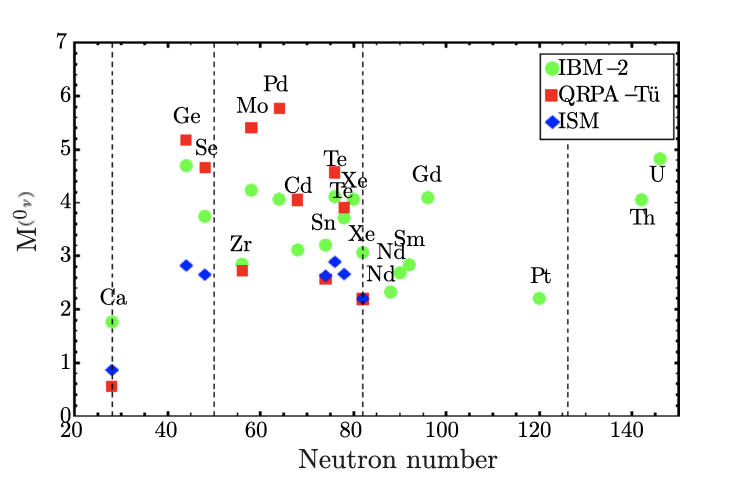
\includegraphics[scale=0.4]{Grafici/NME.png}
	\caption{I valori dei NMEs in funzione del numero di neutroni calcolati secondo i modelli IBM-2~\cite{barea:prc13}, QRPA-T\"{u}~\cite{simkovic:prc13} e ISM~\cite{menendez:npa08}. Figura tratta da~\cite{barea:prc15}.} \label{fig:NME}
\end{figure}



\section{\iflanguage{italian}{Reazioni di DCE e \doppiobeta}{DCE reactions and \doppiobeta}}


%In questo scenario appare evidente la necessità di dedurre dai dati sperimentali nuove informazioni, così da imporre limiti più stringenti ai modelli.  
Da quanto appena detto appare evidente la necessità di imporre limiti più stringenti ai modelli teorici, deducendo dai dati sperimentali nuove informazioni. 
%infatti, nonostante i NMEs non siano direttamente misurabili, sotto opportune condizioni e grazie a modelli teorici appropriati è possibile desumerne il valore tramite misure sperimentali di sezioni d'urto assolute.
In questa prospettiva, le reazioni di \emph{doppio scambio di carica} (Double Charge Exchange, DCE), ovvero le reazioni in cui la carica nucleare cambia di due unità lasciando invariato il numero di massa, si configurano come un potente strumento d'indagine sul \doppiobeta; 
%A causa della bassa sezione d'urto di tali processi, al fine di identificare le reazioni di DCE è essenziale la misura gli spettri energetici con grande risoluzione e le sezioni d'urto assolute ad angoli prossimi a zero.
infatti, sebbene i due processi siano mediati da interazioni differenti, ci sono diverse importanti similarità fra loro.
In primo luogo, gli stati nucleari iniziali e finali del DCE coincidono con quelli del \doppiobeta{}, in quanto in entrambi i casi avviene la trasformazione di due neutroni (protoni) in due protoni (neutroni). 
Un'altra significativa somiglianza riguarda gli operatori di transizione, i quali in tutte e due i processi contengono le componenti a corto range di Fermi, Gamow-Teller e tensoriale di rango-2, con un peso relativo che nelle reazioni di DCE dipende dall'energia incidente. 
Inoltre, in entrambi i casi nel canale intermedio virtuale l'impulso lineare è molto grande, dell'ordine di 100~MeV/c~\cite{barea:prl12}. Questo è un aspetto cruciale, poiché significa che sia le reazioni di DCE sia il \doppiobeta{} sondano stati ad alto impulso della funzione d'onda nucleare, mentre altri meccanismi non ne sono in grado~\cite{puppe:prc11}.

Le reazioni di DCE possono essere uno strumento utile per la comprensione del \doppiobeta{} in quanto permettono di studiare un fenomeno estremamente raro attraverso un meccanismo che, essendo guidato dall'interazione forte, possiede dei tempi caratteristici molto più brevi. 
In aggiunta, il processo di DCE ha il vantaggio di poter essere studiato attraverso misure sperimentali in un laboratorio, in una condizione che consente di tenere sotto controllo alcuni dei parametri fondamentali.
Tuttavia, l'analisi delle reazioni di DCE presenta anche degli inconvenienti: in primis, tali reazioni sono caratterizzate da sezioni d'urto molto basse, tipicamente di alcune decine di nb.
Di conseguenza, per accumulare una statistica sufficiente possono essere necessari lunghi tempi di raccolta dei dati e, a seconda dell'isotopo studiato, fasci di intensità molto grande.
Inoltre, al fine di identificare le reazioni di interesse è essenziale misurare con grande risoluzione e accuratezza sia gli spettri energetici sia le sezioni d'urto assolute ad angoli prossimi a zero. 
%Inoltre, risulta necessario misurare anche gli altri canali di reazione, in modo da  identificare e quantificare i processi di transfer di nucleoni multi-step che concorrono al meccanismo diretto. Questi contributi possono essere minimizzati grazie ad una scelta opportuna del sistema proiettile-target e dell'energia incidente.
Infine, non bisogna dimenticare che eventi così rari sono sommersi da un grande fondo; risulta, dunque, necessario misurare anche gli altri canali di reazione, in modo da poter identificare e quantificare i processi di transfer di nucleoni multi-step che competono con il meccanismo diretto.




\section{\iflanguage{italian}{Il progetto NUMEN}{The NUMEN project}} \label{sez:progetto_numen}

Il progetto NUMEN propone un nuovo metodo per estrarre informazioni basate sui dati sperimentali sui NMEs che entrano in gioco nel calcolo del tasso di dimezzamento del \doppiobeta{}. 
%utilizzando misure accurate di sezioni d'urto di reazioni di DCE indotte da ioni pesanti. 
Per raggiungere tale scopo si intende misurare con grande accuratezza le sezioni d'urto di reazioni di DCE indotte da ioni pesanti, esplorando a diverse energie del fascio incidente \emph{tutti} gli isotopi coinvolti negli esperimenti presenti e futuri sul \doppiobeta{}.
%In particolare, è importante verificare se le sezioni d'urto misurate del DCE sono legate ai NMEs del \doppiobeta{} come una funzione lentamente variabile dell'energia del proiettile e della massa del sistema.%cioè tipo $M^{DCE} \propto f(E_p, A, M^{0 \nu})$
%In tal caso, sarebbe possibile accedere agli elementi di matrice del \doppiobeta{} tramite misure di sezioni d'urto sperimentali. Dal punto di vista teorico, è necessario descrivere accuratamente il meccanismo di reazione, che deve essere fattorizzato in una parte di reazione ed una di struttura nucleare, con quest'ultima a sua volta fattorizzata nel termine del proiettile e in quello del bersaglio.

Il principale, e più ambizioso, obiettivo di NUMEN è l'accesso ai NMEs del \doppiobeta{} attraverso un approccio sperimentale. A tal fine bisogna verificare se gli elementi di matrice del DCE sono legati ai NMEs del \doppiobeta{} come una funzione lentamente variabile dell'energia del proiettile e della massa del sistema.
Qualora questa ipotesi fosse verificata, sarebbe allora possibile dedurre i NMEs del \doppiobeta{} a partire da misure di sezioni d'urto.
% ******* Prima avevo scritto questo:
%Se i risultati sperimentali confermassero che gli elementi di matrice del DCE sono legate ai NMEs del \doppiobeta{} come una funzione lentamente variabile dell'energia del proiettile e della massa del sistema, allora sarebbe possibile dedurre questi ultimi a partire da misure di sezioni d'urto. 
Ciò richiede che il meccanismo di reazione possa essere descritto come il prodotto di un fattore dovuto alla mera reazione e di uno relativo alla struttura nucleare, con quest'ultimo a sua volta fattorizzato in un termine del proiettile e in uno del bersaglio.
%Tale approccio si è dimostrato valido nel caso delle reazioni di singolo scambio di carica (vv. articolo Taddeucci 1987). 
Lo sviluppo di una teoria microscopica coerente della reazione di DCE è, dunque, parte indispensabile del progetto. 
Dal punto di vista sperimentale, la verifica della validità di questa ipotesi richiede la costruzione di una sistematica di dati, che comprenda tutti gli isotopi soggetti al \doppiobeta.
%Sebbene per alcuni casi l'attuale apparato sperimentale possa essere sufficiente, tale studio sistematico richiede l'utilizzo di fasci di intensità molto più elevate di quelle al momento disponibili.
Poiché, come accennato nella sezione precedente, la maggior parte dei processi di DCE presenta sezioni d'urto estremamente basse, tale studio sistematico richiede l'utilizzo di fasci di intensità molto più elevate di quelle al momento disponibili.
In quest'ottica rientra la grande opera di ristrutturazione delle due principali componenti sperimentali: il Ciclotrone Superconduttore (CS) K800 e lo spettrometro magnetico MAGNEX.
%, affrontando le sfide connesse alla ricerca di fenomeni tanto rari, come la bassa sezione d'urto, la grande quantità di background, la necessità di alta risoluzione e sensibilità. 

Altro importante obiettivo di NUMEN consiste nella validazione delle teorie di struttura nucleare che si occupano di calcolare i NMEs del \doppiobeta{};
% ****** Prima avevo scritto:
%; infatti, poiché gli elementi di matrice del DCE e quelli del \doppiobeta{} contengono le stesse funzioni d'onda iniziali e finali e operatori di transizione con struttura simile, la misura di sezioni d'urto assolute può sondare la bontà dei model space adottati dai diversi metodi di calcolo.
infatti, gli elementi di matrice del DCE e quelli del \doppiobeta{} contengono le stesse funzioni d'onda iniziali e finali e operatori di transizione con struttura simile. Se scegliendo un determinato modello di struttura nucleare (con i relativi troncamenti alla funzione d'onda many-body) si trova un buon accordo con i dati sperimentali sulla sezione d'urto del DCE, allora quello stesso model space deve descrivere bene le funzioni d'onda del \doppiobeta.
% Dalla tesi di Ale: "Validare con i dati sperimentali l’applicazione di certi tagli sullo spazio di modello usato nell’analisi dei dati di DCE serve a validare la scelta dello stesso spazio di modello quando l’operatore non è più quello del doppio scambio di carica ma quello del decadimento 0νββ. In questo senso risulta essenziale avere il pieno controllo sulla componente di reazione della sezione d’urto."
Quindi, una volta scelte queste ultime dal confronto con le sezioni d'urto del DCE, le stesse possono essere impiegate per i NMEs del \doppiobeta{}. 

%Infine, NUMEN potrebbe fornire informazioni sulla sensibilità necessaria per la misura del tempo di dimezzamento del \doppiobeta{} a seconda dell'isotopo utilizzato. 
%Infine, NUMEN potrebbe fornire informazioni importanti sui diversi isotopi utilizzati nella ricerca del \doppiobeta{}, perché, facendo il rapporto delle sezioni d'urto assolute misurate negli esperimenti di DCE, si ottiene una stima di quanto il processo sia probabile indipendentemente dal modello adottato. Questa procedura, che consente di ridurre la presenza di eventuali errori sistematici poiché nel rapporto i due contributi si compensano, potrebbe 
Infine, NUMEN potrebbe fornire informazioni importanti sui diversi isotopi utilizzati nella ricerca del \doppiobeta{}, perché il rapporto delle sezioni d'urto assolute misurate negli esperimenti di DCE offre una stima di quanto il processo sia probabile, indipendentemente dal modello assunto. 
%Questa procedura, che consente di ridurre la presenza di eventuali errori sistematici poiché nel rapporto i due contributi si compensano, potrebbe permettere di confrontare
Questa procedura consente di ridurre la presenza di eventuali errori sistematici poiché nel rapporto i due contributi si compensano.
Tale tipologia di analisi potrebbe avere un grande impatto sui futuri esperimenti sul \doppiobeta{}, in quanto potrebbe dare indicazioni su quale isotopo può essere il miglior candidato alla scoperta del processo e sulla sensibilità necessaria per la sua osservazione. 


Gli ambiziosi obiettivi di NUMEN pongono davanti numerose sfide, che richiedono lo sviluppo e l'utilizzo di tecniche innovative sia nel campo teorico sia in quello sperimentale. 
%In particolare, dal momento che il progetto prevede lo studio di tutti gli isotopi candidati al \doppiobeta{}, è necessario utilizzare fasci di intensità molto più alta di quella attualmente disponibile. 
%In questo contesto si inquadra il previsto upgrade delle infrastrutture dei Laboratori Nazionali del Sud (LNS).
%In particolare, dal momento che per studiare tutti gli isotopi candidati al \doppiobeta{} sono necessari fasci ad alta intensità, è fondamentale lo sviluppo di rivelatori capaci di sostenere un alto rate di conteggi.
%In particolare, dal momento che verranno utilizzati fasci ad alta intensità, per il progetto è fondamentale lo sviluppo di rivelatori capaci di sostenere un alto rate di conteggi; infatti, 
%In particolare, la necessità di utilizzare fasci ad elevata intensità rende di fondamentale importanza lo sviluppo di tecnologie di frontiera nell'ambito dei rivelatori ad alto rate di conteggi.
Fra queste, a causa dell'esigenza di utilizzare fasci ad elevata intensità, sono di fondamentale importanza la ricerca e lo sviluppo (R\&D) di tecnologie di frontiera nell'ambito dei rivelatori ad alto rate di conteggi.
%In questo tipo di attività le simulazioni costituiscono un potente strumento per valutare se le performance di un sistema di rivelazione possono soddisfare ai requisiti necessari, evitando così di dedicare tempo e risorse su soluzioni inefficaci.
In questo tipo di attività le simulazioni costituiscono un potente strumento per valutare se una soluzione può soddisfare ai requisiti necessari.

In questo contesto si colloca il ruolo del presente lavoro di tesi, che ha contribuito all'analisi attraverso simulazioni Monte Carlo delle prestazioni di un sistema di rivelazione a stato solido per l'identificazione di ioni pesanti.
%Al fine di validare i risultati della simulazione, è stata svolta un'analisi dei dati sperimentali raccolti in occasione di un test beam svolto ad Aprile 2018, in cui
%I risultati della simulazione sono stati validati con i dati sperimentali del test beam svolto ad Aprile 2018.
Un importante aspetto del presente lavoro verte sulla validazione dei risultati della simulazione attraverso il confronto con i dati sperimentali del test beam svolto ad Aprile 2018, in cui è stata studiata la risposta di un prototipo del sistema di rivelazione simulato.


%All'interno del progetto NUMEN, il presente lavoro di tesi ha contribuito all'analisi attraverso simulazioni Monte Carlo delle prestazioni di un sistema di rivelazione a stato solido per l'identificazione di ioni pesanti.


%L'attuale sistema di rivelazione, basato su pad di silicio, verrebbe danneggiato da tali intensità, quindi servono rivelatori con robustezza alle radiazioni.
%In particolare, è previsto una profonda trasformazione delle due principali infrastrutture sperimentali dell'intero progetto: il Ciclotrone Superconduttore (CS) K800 e lo spettrometro magnetico MAGNEX. 
%Sebbene per alcuni casi 

%L'upgrade dei lns è parte integrante del progetto.

\section{\iflanguage{italian}{L'upgrade dell'apparato sperimentale}{Upgrade of the experimental set-up}} \label{sez:upgrade_apparato}

Come anticipato nella sezione precedente, al fine di studiare in modo sistematico tutti gli isotopi candidati al \doppiobeta{} è necessario utilizzare fasci di intensità molto più alte di quelle disponibili con l'attuale infrastruttura. Dunque, parte integrante di NUMEN è l'upgrade delle due componenti chiave del progetto, il CS e MAGNEX. 
È previsto che, alla fine del processo di ristrutturazione, l'apparato sperimentale possa essere in grado di lavorare con una corrente aumentata di due o tre ordini di grandezza, passando dalle attuali $10^{11}$~pps a circa $10^{13}$~pps.
%Poiché l'aumento della corrente deve essere di due o tre ordini di grandezza
Questo obiettivo può essere raggiunto soltanto a seguito di importanti cambiamenti nelle tecnologie utilizzate nell'estrazione e nel trasporto del fascio, nella realizzazione dei bersagli e nel sistema di rivelazione degli eiettili. 
In particolare, per quanto riguarda quest'ultimo aspetto, i principali cambiamenti previsti sono:
\begin{itemize}
	\item[--] l'aumento della massima rigidità magnetica accettata;
	\item[--] la sostituzione dell'attuale tracciatore a gas, basato su una tecnologia a fili, con un sistema che utilizza i rivelatori Thick-GEM~\cite{cortesi:rsi17};
	\item[--] la sostituzione dell'attuale muro di rivelatori a pad di silicio con una matrice di rivelatori di più piccola taglia e con migliori proprietà di resistenza alle radiazioni;
	\item[--] lo sviluppo di una matrice di rivelatori attorno al bersaglio per la misurazione dei raggi gamma emessi nella diseccitazione degli stati nucleari popolati nelle reazioni di DCE;
	\item[--] l'utilizzo di una nuova elettronica di front-end e di read-out in grado di gestire l'elevato tasso di eventi e l'alto numero di canali previsto.
\end{itemize}
%Dunque, la necessità di sostenere alti rate di particelle porterà ad un profondo cambiamento dell'attuale rivelatore di piano focale (Focal Plane Detector, FPD) di MAGNEX, descritto nel capitolo successivo (\textcolor{red}{aggiungere la sezione}).
Dunque, al fine di raggiungere gli obiettivi preposti da NUMEN è necessaria una profonda trasformazione dell'attuale rivelatore di piano focale (Focal Plane Detector, FPD) di MAGNEX, descritto nel Paragrafo~\ref{sez:progetto_numen}.


%Dei cambiamenti precedentemente elencati particolare attenzione merita quello del tracciatore a gas 
%È importante sottolineare un aspetto dei cambiamenti precedentemente elencati: la sostituzione dell'attuale tracciatore a gas con un sistema 
Dei cambiamenti precedentemente elencati è importante sottolineare un aspetto: il sistema di tracciamento attuale, oltre a fornire accurate informazioni sulla posizione, è sensibile alla perdita di energia degli ioni nel gas. Esso viene, quindi, utilizzato anche come stadio $\Delta E$ per l'identificazione in numero atomico ($Z$) dei prodotti di reazione.
La tecnologia delle Thick-GEM, scelta perché promette buone proprietà di misura della posizione anche in presenza di alti rate, non è invece in grado di dare informazioni sull'energia persa dagli ioni.
Inoltre, gli attuali rivelatori a larga area al silicio, usati per misurare l'energia residua ($ E_{resid} $), non soltanto verrebbero danneggiati da rate così alti, ma sarebbero anche soggetti ad un significativo pile-up a causa delle loro grandi dimensioni.
Di conseguenza, per non diminuire le attuali capacità complessive di identificazione delle particelle (Particle IDentification, PID) è necessario introdurre nel FPD un sistema dedicato a questo scopo.



\subsection{\iflanguage{italian}{Il nuovo sistema di identificazione delle particelle}{The new system of particle identification}} \label{sez:sistema_identif_part}


Il requisito fondamentale che il nuovo sistema di PID deve soddisfare è l'identificazione degli ioni nella regione dell'ossigeno (O), del fluoro (F) e del neon (Ne). 
Oltre a questo, esso deve possedere le seguenti caratteristiche:
\begin{enumerate}
	\item alta resistenza alle radiazioni, in quanto il flusso complessivo atteso sarà dell'ordine di 10\ap{12} $\mbox{ioni}/(\mbox{cm}^2 \cdot \mbox{anno})$;
	\item la risoluzione energetica deve essere sufficientemente buona da garantire una chiara identificazione dei prodotti di reazione di interesse per NUMEN;
	\item il grado di segmentazione deve essere scelto in modo da mantenere la probabilità di eventi con double-hit inferiore al 3\%;
	\item la frazione di volume attivo deve essere sufficientemente alta da ridurre al minimo il fondo costituito dagli eventi con raccolta di carica parziale;
	\item lo spessore dei rivelatori deve riuscire a fermare gli eiettili di interesse in un grande range di energia di incidenza;
	\item i rivelatori devono essere facilmente costruibili e maneggiabili e avere un costo ragionevole.
\end{enumerate}


Dopo aver valutato diverse opzioni, si è scelto di utilizzare un muro di telescopi $ \Delta E - E $ a stato solido.
Negli esperimenti di fisica nucleare questo genere di sistema è tipicamente composto da uno stadio $\Delta E$ sottile al silicio, seguito da un rivelatore spesso al silicio o da uno scintillatore per fermare lo ione.
%La correlazione tra l'energia persa nel primo stadio e l'energia residua depositata nel secondo è legata al numero atomico dello ione rivelato, in accordo con la nota formula di Bethe-Block\cite{knoll:10}.
%Tale tecnica permette l'identificazione degli ioni poiché la correlazione tra l'energia persa nel primo stadio e l'energia residua depositata nel secondo è legata al numero atomico dello ione rivelato, in accordo con la nota formula di Bethe-Block~\cite{knoll:10}.
Tale tecnica permette l'identificazione degli ioni poiché la correlazione tra l'energia persa nel primo stadio e l'energia cinetica totale è legata al numero atomico dello ione rivelato, in accordo con la nota formula di Bethe-Block~\cite{knoll:10}.

Dal momento che, come già detto in precedenza, i rivelatori al silicio non possiedono le proprietà di resistenza alle radiazioni necessarie per il progetto, la scelta è oggi indirizzata verso un telescopio in cui il primo stadio è costituito da un rivelatore sottile (100~$\mu $m) al carburo di silicio~\cite{tudisco:sensors18} (SiC), mentre il rivelatore di stop è uno scintillatore allo ioduro di cesio (CsI) spesso 1~cm.

%Il principale scopo del presente lavoro di tesi è stato la valutazione 
Al fine di verificare se questa scelta possa garantire le performance di PID e la risoluzione energetica necessarie per gli obiettivi del progetto, è stata implementata una simulazione Monte Carlo sulla piattaforma \geant~\cite{agostinelli:nima02,allison:nima16,allison:ieeetns06}.
Tale simulazione, che costituisce l'argomento centrale del presente lavoro di tesi, ha anche lo scopo di valutare la migliore soluzione in termini di granularità, stimando il numero di eventi con raccolta di carica incompleta.








\section{\iflanguage{italian}{Le fasi del progetto}{The phases of the project}}

Il progetto NUMEN è articolato in quattro fasi, di cui verranno esposti i tratti più importanti. 

La \emph{Fase 1}, già completata, ha dimostrato, grazie all'esperimento pilota \ce{^{40}Ca}(\ce{^{18}O},\ce{^{18}Ne})\ce{^{40}Ar}, che è possibile estrarre informazioni sulle funzioni d'onda nucleari del \doppiobeta{} tramite lo studio di reazioni di DCE.

La \emph{Fase 2}, attualmente in corso, prevede lo svolgimento di una campagna sperimentale su alcuni isotopi di interesse, scelti come compromesso tra la rilevanza di tali isotopi per gli esperimenti sul \doppiobeta{} e le esigenze tecniche. I primi sistemi oggetto di studio sono stati $^{116}\mbox{Cd}\,  - \, ^{116}\mbox{Sn} $ e $^{76}\mbox{Ge}\,  - \, ^{76}\mbox{Se} $, sondati attraverso le reazioni (\ce{^{20}Ne}, \ce{^{20}O}) e (\ce{^{18}O}, \ce{^{18}Ne}) per esplorare il meccanismo di DCE in entrambe le direzioni. Prossimamente verrà effettuato un esperimento sulla reazione \ce{^{48}Ti}(\ce{^{18}O},\ce{^{18}Ne})\ce{^{48}Ca}. 
%Durante questa fase verrà anche ottimizzata la strategia di analisi dei dati.
Della Fase~2 fa parte anche l'attività di R\&D su rivelatori, materiali e tecnologie precedentemente descritta.

La \emph{Fase 3} comprende sia lo smontaggio dell'attuale apparato sperimentale sia l'assemblaggio del nuovo. In questa fase avrà luogo anche l'upgrade del CS e della linea di trasporto. La durata prevista è di 18 - 24 mesi.
%La \emph{Fase 3} è dedicata all'upgrade del CS e di MAGNEX: in questa fase 


La \emph{Fase 4} prevede una serie di campagne sperimentali che, grazie alle acquisite condizioni di alta intensità del fascio, comprenderà tutti gli isotopi di interesse per il \doppiobeta{}. 
Questa fase sarà dedicata al calcolo della sezione d'urto assoluta di DCE. Se l'analisi teorica sarà riuscita a sviluppare una descrizione microscopica delle reazioni di DCE, allora sarà possibile avere accesso ai NMEs del \doppiobeta{}, principale obiettivo di NUMEN.










\clearpage




%\cleardoublepage
%\phantomsection
%\chapter*{\iflanguage{italian}{Conclusioni}{Conclusions}}
%\addcontentsline{toc}{chapter}{\iflanguage{italian}{Conclusioni}{Conclusions}}

%\lipsum[20]


\cleardoublepage
\phantomsection
\addcontentsline{toc}{chapter}{\iflanguage{italian}{Bibliografia}{Bibliography}}
\bibliographystyle{mprsty}
\bibliography{biblio}


%\cleardoublepage
%\phantomsection
%\chapter*{\iflanguage{italian}{Ringraziamenti}{Acknowledgements}}
%\addcontentsline{toc}{chapter}{\iflanguage{italian}{Ringraziamenti}{Acknowledgements}}

%\lipsum[20]

\end{document}




